%-----------------------------
% CHAPTER 2: State-of-the-art
%-----------------------------

\chapter{State-of-the-art}

\label{chapter02}

Since this project is not oriented for \company\ users but the company itself, the \textit{\nameref{chapter02}} relates to services inside \company. Even so, a brief explanation about other metasearch engines would help to find the gap this project is developed.

%-----------------
%   SECTION 2.1
%-----------------

\section{Fare aggregators and metasearch engines}

\subsection{Google Flights}

In the last years Google Flights has became the main competitor of \company. The new version is very fast and has a complete new interface, following Material Design guidelines.
\\\\
Google is one of the top tech companies worldwide and has a lot of different platforms. It is a competitor to be aware of, the integration with Gmail, Google Calendar and Android OS makes Google Flight a part of Google's ecosystem. The traveler may feel comfortable.

\subsection{Kayak}

Kayak has always been the main competitor, both companies started in 2004. Unlike \company, Kayak started with Flights, Hotels and Car hiring. \company\ added those two extra search engines between 2013 and 2014.

\subsection{Expedia}

Launched in November 1998, is one of the oldest fare aggregator and metasearch engine. Apart of its own website, is also a \company\ provider. Some of the prices are taken from Expedia and sometimes the user is redirected to their website to finish their purchase.

%-----------------
%   SECTION 2.2
%-----------------

\section{\company\ services}

In \company\ the user has never been a product, in fact, one of the statements of \company's culture says \textit{Traveler != Product}\cite{the_road_ahead}.
\\\\
There has never been a project getting value from user information because it does not follows the company culture, so the definition of the problem and the scope of the project must be very accurate to ensure it is fulfilling with \company's strategy\cite{skyscanner_strategy}.

\subsection{Marketplace Engine} \label{mp_engine}

This tribe is formed by five squads, those constantly work to improve the routes and pricing service all along with an efficient search.
\\\\
Marketplace Engine works with data \textit{from the provider to the user}. In other words, it just serves \textbf{information to the user} but does not get any from him/her. All five squads take all the \textbf{data from providers}.

\begin{figure}[H]
\centering
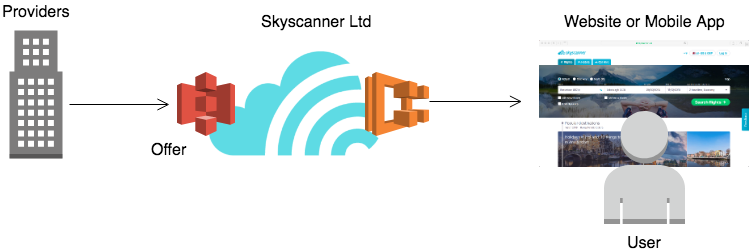
\includegraphics[scale=0.45]{diagrams/state-of-the-art-tribes-marketplace-engine.png}
\caption{Simple explanation of Marketplace Engine data flow.}
\end{figure}

\subsection{Data tribe} \label{data_tribe}

In the other hand, Data tribe has a lot of squads with services used to collect \textbf{data from user's activity}. The flow of the information is \textit{from the user to \company}.

\begin{figure}[H]
\centering
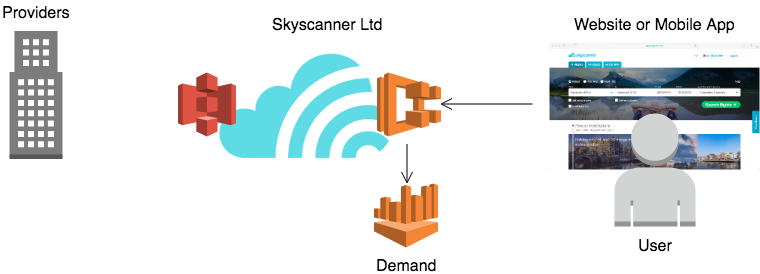
\includegraphics[scale=0.45]{diagrams/state-of-the-art-tribes-data-tribe.png}
\caption{Simple explanation of Data Tribe data flow.}
\end{figure}

\subsection{The gap}

There is no tribe or squad that works with both \textbf{data sources}: Providers and Users. And here is where the \textit{\thesistitle} will be.

\begin{figure}[H]
\centering
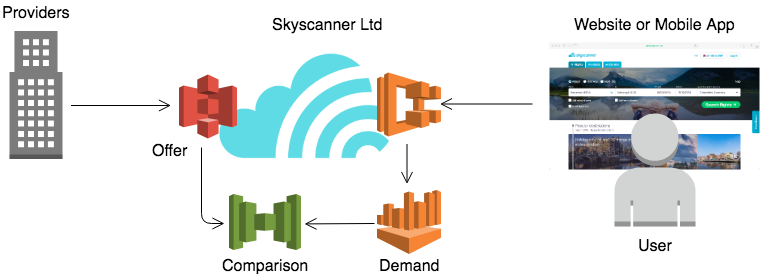
\includegraphics[scale=0.45]{diagrams/state-of-the-art-tribes-comparison.png}
\caption{First approach of the \thesis data flow.}
\end{figure}

%-----------------
%   SECTION 2.3
%-----------------

\section{Resources} \label{resources}

\company\ is already in the air, it is working and has been working for more than ten years. In the past two years it has been migrating all their services to Amazon Web Services\cite{aws}.
\\\\
Amazon Web Services have a lot of available different services in it for different purposes. The services that will be used or important for this projects are\footnote{All the resources are well defined in chapter \nameref{chapter06} on page \pageref{chapter06}}:

\begin{itemize}
    \item Compute
    \begin{itemize}
        \item Lambda
        \item Batch
        \item ECS: Elastic Container Service
    \end{itemize}
    \item Storage and Database
    \begin{itemize}
        \item S3: Simple Storage Service
        \item DynamoDB: Dynamic Database
        \item RDS: Relational Database Service
    \end{itemize}
    \item Analytics
    \begin{itemize}
        \item Athena
        \item EMR: Elastic MapReduce
        \item Data Pipeline
    \end{itemize}
    \item Others
    \begin{itemize}
        \item CloudFormation, Management Tools
        \item API Gateway, Networking \& Content Delivery
        \item Simple Notification Service, Application Integration
    \end{itemize}
\end{itemize}



